Suppose that we have a four stage pipeline where each instruction takes only one cycle. Let $a$ and $b$ be two instructions with an R/W dependency, i.e. instruction $b$ uses a value that is defined by instruction $a$. During the first cycle, instruction $a$ is fetched from Instruction Memory (IMEM). In the second cycle, instruction $a$ selects the operands from the RF, and instruction $b$ is fetched from IMEM. During the third cycle, instruction $a$ is in the execution stage, while instruction $b$ selects the operands that it needs. During the fourth cycle, instruction $a$ is in the WB stage, where it writes the result back to the RF, and instruction $b$ is in the execution stage.

Without bypassing, the result of instruction $a$ will be available only after it is written back. On the other hand, when we do have a bypass network, we may forward the result of an instruction to another instruction. In our example, we have forwarded the result of instruction $a$ directly to the operand of instruction $b$, as indicated by the vertical arrow that goes from the first to the second instruction in Figure \ref{fig:bypass_principle}. A result of an instruction may be accessed a cycle earlier when we compare with and without bypassing, however, the target architecture has either explicit or implicit bypassing, which both access a result of an instruction a cycle early. So, in terms of cycles, it makes no differences whether to use explicit or implicit bypassing. However, as you will see later, explicit bypassing has an advantage over implicit bypassing.

\begin{figure}[H]
\centering
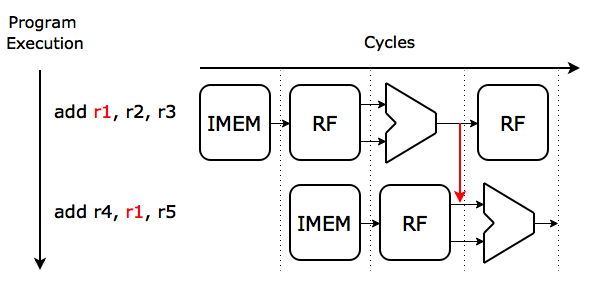
\includegraphics[width=.6\textwidth]{figures/bypassing_principle/05_bypassing_principle}
\caption{Illustration of bypassing and software pipelines in general.}
\label{fig:bypass_principle}
\end{figure}

With bypassing, we have wires that connect outputs of EX stage to the ID stage and we have this for each bypass source. 

\section{Implicit Bypassing}
With implicit bypassing, we have wires that connect the outputs from EX stage to the ID stage, as illustrated in Figure \ref{fig:impl_bypass_principle}. Furthermore, we also have wires that go from the WB stage to the ID stage, however, this is not shown in this example. To detect bypasses, the HW matches whether the operands of the currently issued instruction to the destination address of previously issued instructions. If we have a match, and the result is still available in the pipeline, we can then bypass it. We have a mux that controls which inputs are used, i.e. a value from a register, or a value from a bypass. The bypass detection hardware is in control which of these values is selected.

\begin{figure}[t]
\centering
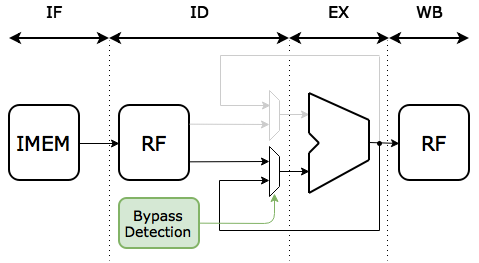
\includegraphics[width=.5\textwidth]{figures/impl_bypassing_principle/03_implicit_bypassing_principle}
\caption{Illustration that shows the basic principles of implicit bypassing.}
\label{fig:impl_bypass_principle}
\end{figure}

\section{Explicit Bypassing}
For explicit bypassing, we have similar wires that connect outputs of EX stage to the ID stage as we have in implicit bypassing. However, with explicit bypassing the compiler is responsible for detecting when we can bypass the result of an instruction. In Figure \ref{fig:exp_bypass_principle_r} we show that the control signal to the mux, that selects the input from a register or from a bypass, is now controlled by the compiler. The compiler encodes this information in an instruction. This way, during instruction decoding, the control signal is immediately available. Furthermore, we have a read-enable flag on the register file. If we then want to take the data from a bypass, we can set this value to zero. This way, we can avoid speculative reads accesses from the RF. We use the same signal from the ID stage, to control the read-enable on the register file and the signal that controls the mux. 

\begin{figure}[H]
\centering
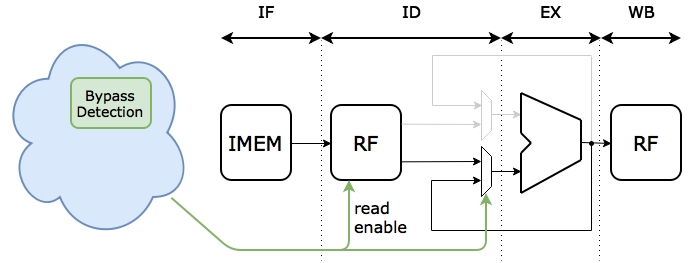
\includegraphics[width=.7\textwidth]{figures/expl_bypassing_principle/01_explicit_bypassing_principle}
\caption{Illustration that shows the basic principles of explicit bypassing, read enabled port on RFs to avoid unnecessary reads.}
\label{fig:exp_bypass_principle_r}
\end{figure}

We can use the liveliness information during compilation to determine whether a variable is live after it is used. If the variable is not live after it is used often indicated by a kill of a variable, we can disable the write on the register, since it will not be needed anymore. Figure \ref{fig:exp_bypass_principle_rw} illustrates this by adding a write-enable flag on top of the read-enable that was already present from Figure \ref{fig:exp_bypass_principle_r}. Adding a write-enable flag allows us to avoid speculative write accesses to the RF.

\begin{figure}[t]
\centering
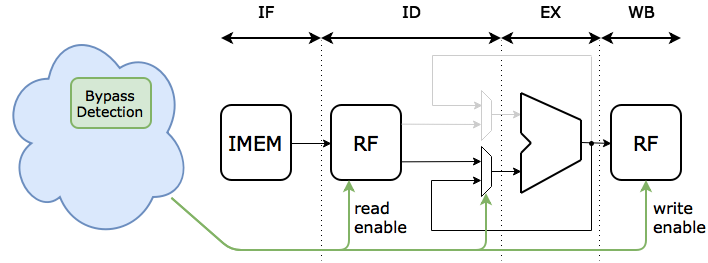
\includegraphics[width=.7\textwidth]{figures/expl_bypassing_principle/02_explicit_bypassing_principle}
\caption{Illustration that shows the basic principles of explicit bypassing, read enabled port on RFs to avoid unnecessary reads and write enable port to avoid speculative writes.}
\label{fig:exp_bypass_principle_rw}
\end{figure}

A significant difference between explicit and implicit bypassing is that some write accesses to the register file may be avoided for explicit bypassing, while this is can not be done with implicit bypassing.

In general, the result of an instruction will remain in the pipeline  scheduled in the future, in order to see whether the result of an operation will be used later on, which is not possible at runtime.

%%%%%%%%%%
%\section{Bypass Sources}

The target architecture has operand isolation, which we mentioned in Chapter \ref{sec:processor}. Because of this, the output of the function units do not toggle, i.e. are only calculated when the operand registers change. This has as a side effect that when a function unit is not used, the output register remains the same. This means that an instruction can be bypassed, as long as we do not use the function unit on which it was executed. We have given the bypass sources for our architecture below, in Table \ref{table:bypass_alias}. Here we have provided all bypass sources for the four stage and five stage pipeline

\begin{table}[H]
\caption{Alias for each bypassing source, $BP\_src$ in Figure \ref{fig:4_stage} and Figure \ref{fig:5_stage}.}
\begin{center}
\begin{tabular}{@{}llll@{}}
\toprule
\multirow{2}{*}{\textbf{Register:}} & \multirow{2}{*}{\textbf{Bypass source:}} & \multicolumn{2}{c}{\textbf{Alias}:} \\ \cline{3-4}
 & & \textbf{4 stages} & \textbf{5 stages} \\
\hline
\emph{r27} & $BP\_src27$ & N/A & ALU1 \\ 
\emph{r28} & $BP\_src28$ & LSU & LSU \\
\emph{r29} & $BP\_src29$ & MUL & MUL \\ 
\emph{r30} & $BP\_src30$ & ALU & ALU2 \\
\emph{r31} & $BP\_src31$ & WB & WB \\
\bottomrule
\end{tabular}
\end{center}
\label{table:bypass_alias}
\end{table}%

%%%%%%%%%%%%

We will now show with an example that avoiding speculative write accesses may reduce Register Pressure (RP).

%TODO: move this to a better place, or explain this in one of the previous sections
%this being that we have multiple bypassing sources, we specify them as if they were a register, and the following registers map to the following bypassing sources.
%One from each FU, one from WB and an additional one from blala
%With automatic bypass we actually always bypass from WB, because otherwise each instruction would take one more cycle. Namely one or two execution stages and a wb stage after which the result is the register.
%With explicit bypassing the compiler can avoid some accesses to RFs by explicitly specifying the datapath.

%Connect to TTA architectures, use findings of Johan Janssen.

%Show the need for this like done in Johans' paper. (and in lucs paper)

%Different approches
% - Naive implementation
% - Scheduling pass to automate it
% - Combine RA and scheduling to do it better.
% - Use LLVMs way to describe explicit bypassing, namely targetItinirary.td

\begin{lstlisting}[caption=Example code fragment where no bypassing is specified., label=lst:nobypass]
mul <@\textcolor{red}{r1}@>, r2, r3
add r4, <@\textcolor{red}{r1}@>, r5
\end{lstlisting}

Listing \ref{lst:nobypass} shows a code fragment with a multiplication and an addition. We have a flow dependent dependency. Namely, the result of the multiplication is used by the addition.

\begin{lstlisting}[caption=Example code fragment avoiding a read access., label=lst:operandbypass]
mul <@\textcolor{red}{r1}@>, r2, r3
add r4, <@\textcolor{red}{MUL}@>, r5
\end{lstlisting}

In Listing \ref{lst:operandbypass} we have replaced the use of $r1$ with $MUL$. This indicates that we do not take the first operand from the RF, but from a bypass instead. Since we obtain the result of the multiplication from the bypass network, we do not require a read access to $r1$ anymore.
%This is also done for the implicit bypassing approach, however since we have more bypass sources for the explicit bypassing variant, we expect that operand bypassing is done more aggressively.

\begin{lstlisting}[caption=Example code fragment avoiding a read and a write access., label=lst:fullbypass]
mul <@\textcolor{red}{--}@>, r2, r3
add r4, <@\textcolor{red}{MUL}@>, r5
\end{lstlisting}

When the result of $r1$ is not needed anymore, for example, the live range of $r1$ spans no further than this addition, the write access can be avoided. By specifying $--$ as the destination, the result will not be written back, as illustrated in Listing \ref{lst:fullbypass}. Register $r1$ is now completely removed from the example, effectively freeing that register. We have now reduced RP by one since we require one less register. The freed register can be used for other calculations, which may lead to a higher performance.

%%%%%%%%%%%%%%%%%%%%%%%%%%%%


%HERE WE SHOW ALL DIFFICULT CASES, i.e. First instruction of loop body is bypassed from last instruction of loop body.
\section{Joint Point Issue}
In the following example, we will illustrate a special case that may be taken into consideration.

\begin{lstlisting}[caption=Example code fragment where bypassing over backedge of a loop iteration is not possible., label=lst:bypassloop1]
      lw <@\textcolor{red}{r6}@>, r10, 5
loop: 
        <@\raisebox{-1pt}[0pt][0pt]{$\vdots$}@>
      
      sfeq <@\textcolor{red}{r6}@>, r0
      bnf loop
      addi <@\textcolor{red}{r6}@>, <@\textcolor{red}{r6}@>, -1

        <@\raisebox{-1pt}[0pt][0pt]{$\vdots$}@>
\end{lstlisting}

When we access the loop counter for the first time in Listing \ref{lst:bypassloop1}, $r6$ can be bypassed from the $LSU$. However, in consecutive iterations, we would bypass it from the $ALU$ instead. Listing \ref{lst:bypassloop2} shows that adding an instruction before entering the loop allows us to bypass the value in consideration. We may profit from this if a lot of loop iterations are processed.

\begin{lstlisting}[caption=Example code fragment where bypassing over the backedge of a loop iteration is possible., label=lst:bypassloop2]
      lw <@\textcolor{red}{--}@>, r10, 5
      add <@\textcolor{red}{r6}@>, <@\textcolor{red}{LSU}@>, 0
loop: 
        <@\raisebox{-1pt}[0pt][0pt]{$\vdots$}@>
      
      sfeq <@\textcolor{red}{ALU}@>, r0
      bnf loop
      addi <@\textcolor{red}{--}@>, <@\textcolor{red}{r6}@>, -1

        <@\raisebox{-1pt}[0pt][0pt]{$\vdots$}@>
\end{lstlisting}

%TODO: leg dit eens fatsoenlijk uit joh
Here we want to apply bypassing to bypass the result of the last add instruction in the loop before we branch to the first instruction in the loop. However, when we go in the loop for the first time, $r6$ comes from the LSU instead of the ALU. Therefore, sometimes it is necessary to insert an instruction before we enter a loop to bypass over loop iterations.

%\section{Proposed Approaches}
%We will investigate in different approaches to implement software bypassing on top of the SIMD architecture within LLVM. Each of these approaches will be evaluated. The kernels that we will use as means of evaluation are discussed in Chapter \ref{sec:benchmark}.

%\begin{enumerate}
%\item Naive approach in which we will add a pass on top of the existing scheduler to apply software bypassing whenever possible. In this approach, explicit datapaths are created after scheduling and register allocation.
%\item Use LLVMs framework to express the processors pipeline stages and bypassing sources. This way LLVM will apply software bypassing. This will be a good reference for our final approach.
%\item Implement a bypass aware combined scheduling and register allocation algorithm. We need to investigate what steps need to be taken to implement a custom scheduler in LLVM.
%TODO: introduce the need for combined scheduling and RA..... 
%\end{enumerate}
%Incorporate notes from 21/22 februar, write a long text to discuss all of them. This way we have motivation for each of the proposed solutions.

%TODO: make example for each approach.

%\section{Method of Evaluation}\label{sec:benchmark}
%Discuss the kernels that we will use to evaluate the different approaches. We will use RTL synthesis to emulate the processors behaviour on certain kernels and model the energy consumption for each of the approaches, for the transparent bypassing variant, and finally for a by hand optimized and bypassed variant. This should give us an "optimal" energy reduction compared to the energy reduction that we achieved, with transparent bypassing as reference.


